The equivalence principle serves as the foundational insight for interpreting gravity in geometric terms. It identifies the universality of free fall as a property of spacetime rather than a consequence of force interactions between masses. In this view, gravitational acceleration arises from the nature of spacetime itself.

In its simplest formulation, the weak equivalence principle states that all freely falling bodies released from the same point with the same initial velocity trace out identical trajectories, regardless of their mass, internal structure, or chemical composition. No deviation has been observed, even across experiments involving diverse materials and precision measurements.

This regularity, empirically established since Galileo’s observations, implies that gravitational acceleration is independent of any material-specific parameters. It does not vary with mass, charge distribution, or binding energy, and thus cannot be attributed to internal mechanisms of the falling object.

Because different materials follow identical free-fall trajectories, the determining factor cannot reside in any internal property of the objects themselves. The motion must be governed by features external to the material body. In this framework, the path of a falling object is taken to reflect the geometry of spacetime — specifically, the metric field — rather than any material-dependent force law.

The strong equivalence principle generalizes the uniformity of free fall to the behavior of physical laws themselves. It asserts that in any local region of spacetime, the effects typically attributed to gravity can be eliminated entirely by choosing an appropriate frame of reference — specifically, one that is freely falling with respect to the surrounding mass distribution.

Within such a frame, spacetime curvature becomes negligible. The geometry flattens to first order, and all physical processes proceed as they would in the absence of gravitation. Mechanical systems evolve according to Newton’s laws, electromagnetic fields obey Maxwell’s equations in vacuum, and the motion of particles is governed by the inertial character of special relativity.

This locality condition introduces a precise operational statement: although spacetime may be globally curved due to the distribution of matter and energy, it admits neighborhoods that are indistinguishable from flat Minkowski space. No experiment confined to a sufficiently small free-falling laboratory can reveal the presence of gravitation through deviations from special-relativistic predictions.

Einstein’s elevator thought experiment provides a concrete illustration of the strong equivalence principle. Consider an elevator in free fall, sealed from external observation. An observer inside releases an object from rest relative to the elevator. The object remains at rest relative to the cabin, as though floating weightlessly. A beam of light, emitted from one wall to the opposite, travels in a straight line. No outcome of any experiment conducted within this enclosure depends on the external gravitational field.

This conclusion holds across all physical domains. Mechanical pendulums, electromagnetic resonators, radioactive decay rates, and interference patterns behave identically to those in an inertial frame situated in the absence of gravity.

The indistinguishability reflects a physical equivalence: free fall in a gravitational field and inertial motion in flat spacetime produce identical conditions for the evolution of all physical systems, provided the region under consideration is sufficiently small to neglect tidal effects.

The equivalence principle applies strictly to infinitesimal regions of spacetime. Over small enough domains, the effects of curvature vanish, and local physics is indistinguishable from that of special relativity. However, as the domain is extended, small deviations accumulate. The presence of spacetime curvature becomes detectable when comparing outcomes across separated locations, even if each local region individually admits a flat approximation.

These deviations appear in multiple observable forms. Clocks positioned at different gravitational potentials accumulate proper time at different rates. Nearby free-falling trajectories, initially parallel, may converge or diverge depending on the spacetime geometry. The presence of tidal effects — variations in relative acceleration across an extended object — provides direct physical evidence that the background is not flat.

A local inertial frame is defined by the absence of proper acceleration and by the applicability of special-relativistic laws. Within such a frame, light travels in straight lines, and ideal clocks advance at constant rates. These conditions are satisfied when the spacetime geometry, as described by the metric tensor, becomes indistinguishable from that of flat spacetime at a single point. More precisely, the components of the metric can be matched to those of special relativity at that location, with any deviations becoming apparent only at second order in spatial or temporal displacement from the point of comparison.

When local inertial frames are established at distinct locations and compared, observable discrepancies emerge. Clocks positioned at different altitudes accumulate proper time at unequal rates, and vectors transported between frames fail to align consistently. These effects reveal that no single coordinate system can render the metric flat across extended regions. The mismatch is not a coordinate artifact but a consequence of intrinsic curvature, encoded in the second derivatives of the metric tensor.

The presence of spacetime curvature becomes operationally meaningful when comparing local measurements across finite regions. One method involves tracking the motion of free-falling particles that begin at rest relative to each other. In flat spacetime, such particles would maintain their initial separation. In a curved geometry, they may gradually drift apart or move closer together, depending on the surrounding mass distribution. This behavior is known as geodesic deviation, and it reflects how curvature alters the shape of nearby inertial paths. The rate and direction of this deviation are determined by the local curvature tensor, which measures how much the rules of parallel transport fail to preserve vector separation.

Another method involves exchanging signals between observers located at different gravitational potentials. If two identical clocks are placed at different altitudes and used to emit pulses of light at regular intervals, the receiver will measure those intervals as changing. Light sent upward from a lower potential arrives with a longer wavelength, an effect known as gravitational redshift. Light sent downward is blueshifted. These outcomes are not due to any stretching or compression during transmission. Instead, they reflect the changes in the flow of timw. Each clock accumulates proper time according to its location in the metric field, and the discrepancy in rates reveals a persistent gradient in temporal flow.

The spacetime metric is the mathematical object that defines how durations and distances are assigned to events. It encodes the geometry of both time and space, determining how clocks tick, how lengths are measured, and how objects move when no forces are applied. In flat spacetime, the metric is constant, and these assignments match those of special relativity. In curved spacetime, the metric components vary with position, and this variation underlies observable gravitational phenomena.

A helpful analogy comes from curved surfaces. Imagine two travelers walking north from the equator along different lines of longitude. Their paths begin parallel and appear straight locally, yet they eventually converge at the pole. The meeting point is not due to any force between them but to the surface’s geometry. In spacetime, freely falling objects can similarly start with zero relative velocity and later converge or diverge, not because of an interaction, but because the spacetime metric changes from point to point. The curvature of the manifold governs how local inertial paths extend and how global structure emerges from local geometry.

Among the components of the metric, the one labeled \( g_{00} \) controls how proper time accumulates for stationary observers. When \( g_{00} \) differs between locations, the same interval of coordinate time corresponds to different amounts of actual time experienced. This variation causes gravitational time dilation. While spatial curvature contributes to global phenomena such as lensing and tidal effects, the local behavior of clocks and the direction of free fall are determined primarily by the gradient of \( g_{00} \). It is the variation in the rate of time's passage that produces the familiar experience of gravitational acceleration.

A geodesic is the path a freely moving object traces through spacetime. In special relativity, this path is a straight line at constant velocity. In general relativity, a geodesic is defined as the trajectory along which proper time is extremized. The metric determines what counts as a straight path in this generalized sense.

In a gravitational field, geodesics are not straight in space. Near Earth, for example, an object released from rest accelerates downward because proper time accumulates more slowly near the surface. The object curves toward regions where time flows more slowly. The acceleration we observe is the projection of this curved spacetime path into spatial coordinates.

Free-falling objects follow these geodesics precisely. The direction of motion is set by the gradient of proper time. Orbits, local falling, and light deflection all follow the same rule: objects move in the direction that locally maximizes elapsed time. The metric defines both temporal rates and spatial separations, and these together determine how free motion unfolds.

That clocks at different altitudes tick at different rates is a direct consequence of the metric, specifically of the spatial variation in \( g_{00} \). A fixed interval of coordinate time corresponds to more or less proper time depending on position. This difference has been confirmed using atomic clocks aboard airplanes, satellites, and mountaintops, and it is essential for GPS accuracy.

This same variation governs motion. A freely falling object always moves toward regions of slower time. Consider an apple hanging from a tree. While attached, it resists the geodesic assigned to its position. Once the stem breaks, it is no longer constrained. It enters inertial motion, and its path curves downward because proper time accumulates more slowly below.

As the apple descends, the gradient of proper time changes continuously. The trajectory adjusts to follow the direction where time advances least quickly. The resulting curvature in its path is what we perceive as acceleration. This acceleration is not caused by any external agent. It is not carried by particles, nor transmitted through a field in the usual sense. The motion arises from the metric itself. Spacetime tells the apple how to move by encoding how time flows from point to point.

Spatial curvature plays a role in large-scale effects, including lensing and tidal stress. But the immediate cause of falling is temporal. The non-uniform flow of time across space determines the direction of motion. Gravity, in this formulation, is the visible effect of unequal clock rates embedded in the geometry of spacetime.


\begin{commentary}[Falling Into Slower Time]

The realization that gravity arises from differences in the rate of time’s passage, rather than from any applied force, marks a profound shift in understanding. This perspective is mathematically well-defined and supported by high-precision experiments, but it remains difficult to visualize in intuitive terms.

One of the most common teaching tools, the rubber sheet analogy, shows mass distorting a two-dimensional surface. Smaller objects curve toward the resulting indentation, mimicking planetary orbits. Although this conveys the idea that mass alters geometry, it centers attention on spatial curvature. In general relativity, however, the dominant effect responsible for gravitational motion is not the curvature of space, but the variation in proper time from place to place. Time flows more slowly deeper in a gravitational field. This gradient governs how free-falling objects move. The metric of space may also curve, but the decisive influence on motion is temporal.

This is, for me, a \textit{fantastic} observation. An apple falls from a tree not because it is pulled downward, but because time flows slightly faster at the top of the tree than at the bottom. Once released, the apple is no longer constrained. It follows a trajectory through spacetime that maximizes the amount of proper time experienced along the way. The curve of this path is determined by how the clock rate changes with altitude.

In everyday reasoning, we often think of objects as taking the shortest route through space. But in general relativity, freely falling objects follow the most direct path through spacetime as a whole. This path is not defined by distance alone. It is shaped by how the passage of time varies from point to point, even when those variations are imperceptible without careful measurement.

\end{commentary}


\thispagestyle{empty}
\begin{figure}[p]
\centering
\fbox{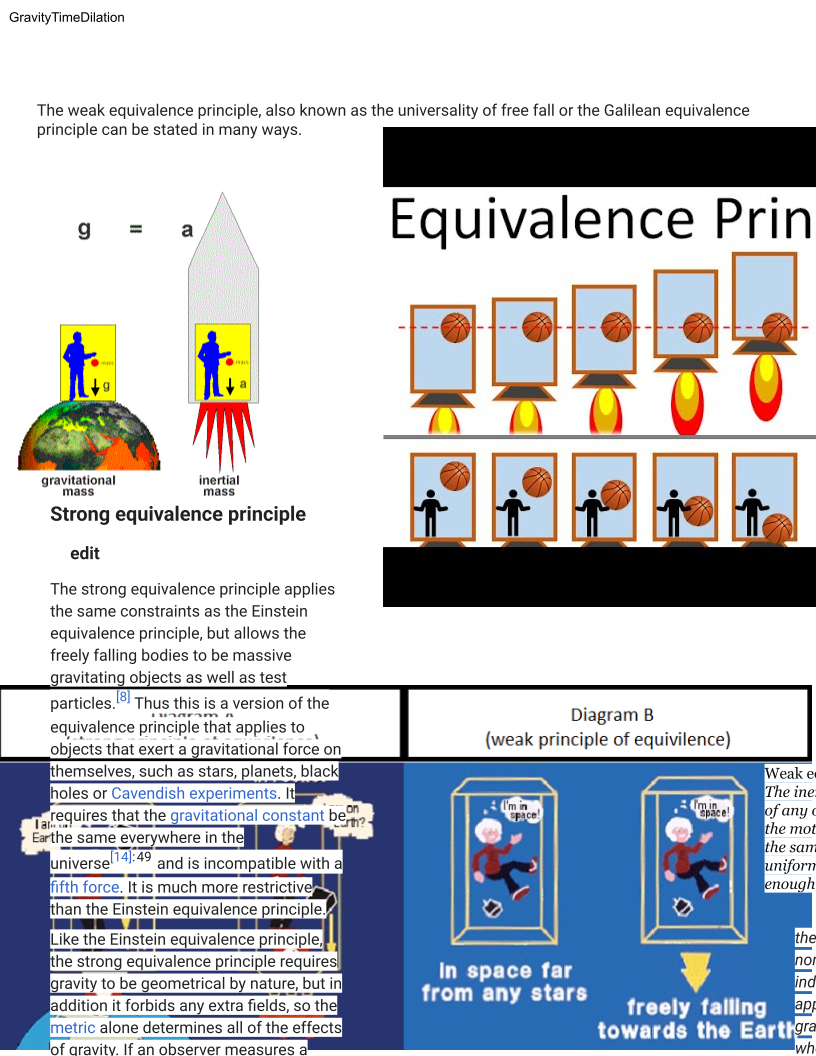
\includegraphics[width=\textwidth,height=\textheight,keepaspectratio]{06_GravityTimeDilation/equiv_illus.png}}
\end{figure}